Модуль Remap является частью жидкоаргонового сигнального процессора LASP (рис. \ref{fig:remap_lasp}) и в первую очередь предназначен для организации упорядочивания входных данных в соответствии с геометрией детектора.\par
\begin{figure}[ht]
    \centering
    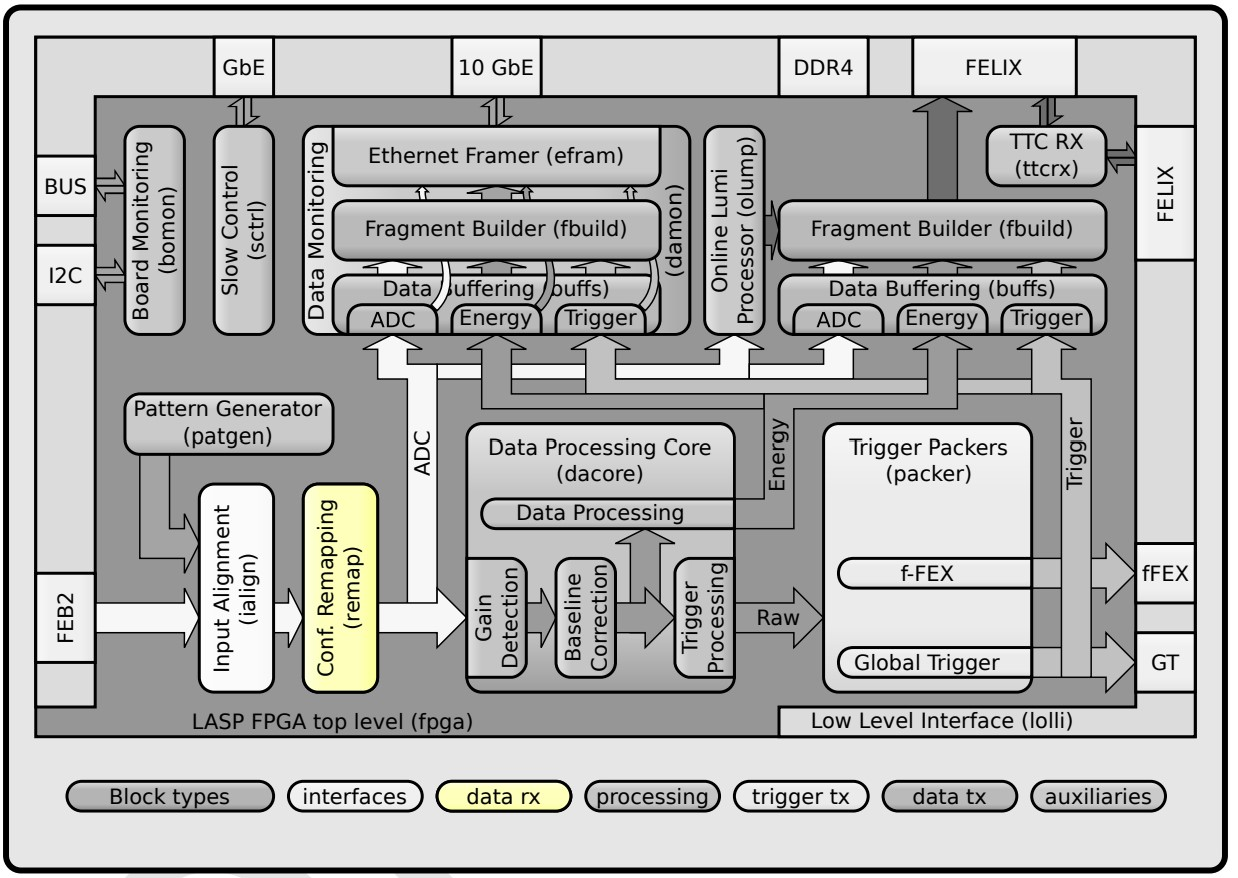
\includegraphics[width=0.8\linewidth]{remap_lasp.png}
    \caption{Схема расположения модуля Remap в общей структуре сигнального процессора LASP}
    \label{fig:remap_lasp}
\end{figure}\par
Remap компонент должен реализовывать приём поступающей информации и формировать из неё набор выходных каналов данных, в каждом из которых обязаны передаваться значения АЦП, выбранные из входных каналов в соответствии с установленной конфигурацией, в определённом порядке, также согласно конфигурации. Требование конфигурируемости через интерфейс медленного контроля является очень важным, поскольку для обработки огромного потока данных с калориметров предполагается размещение значительного количества модулей LASP, в каждом из которых схема перестановок может отличаться. Более того, даже в рамках одной системы располагается несколько таких экземпляров, так что настройка параметров каждого модуля на этапе компиляции совершенно не приемлема.\par
Как упоминалось ранее, сигнальный процессор LASP проектируется в двух вариантах, так называемые медленная и быстрая опции. В любом варианте система работает с 88 входными каналами, поступающими на частоте $f_{feb} = 320$ МГц, которые преобразовываются либо в 64, либо в 43 выходных канала данных соответственно, передающихся на частоте $f_{core}$. Это преобразование производится непосредственно с помощью модуля Remap, таким образом, следующим важным требованием является реализация корректного перевода сигналов между тактовыми доменами. Кроме того, поскольку LASP является системой, передающей данные в триггер, то существуют конкретные ограничения по задержке данных: 1,6 времени между столкновениями пучков или 40 нс.\par

\subsection{Архитектура модуля}
Основополагающим подходом в проектировании модуля конфигурируемой перестановки \texttt{remap} является создание таких элементарных устройств, которые способны принимать на вход весь требуемый объём данных и формировать из него лишь один выходной канал. Это обеспечивает высокую гибкость в масштабировании, поскольку в таком случае реализация необходимого количества выходных каналов достигается простой репликацией подобных структур, как это показано на рисунке \ref{fig:remap_replication}.\par

\begin{figure}[ht]
    \centering
    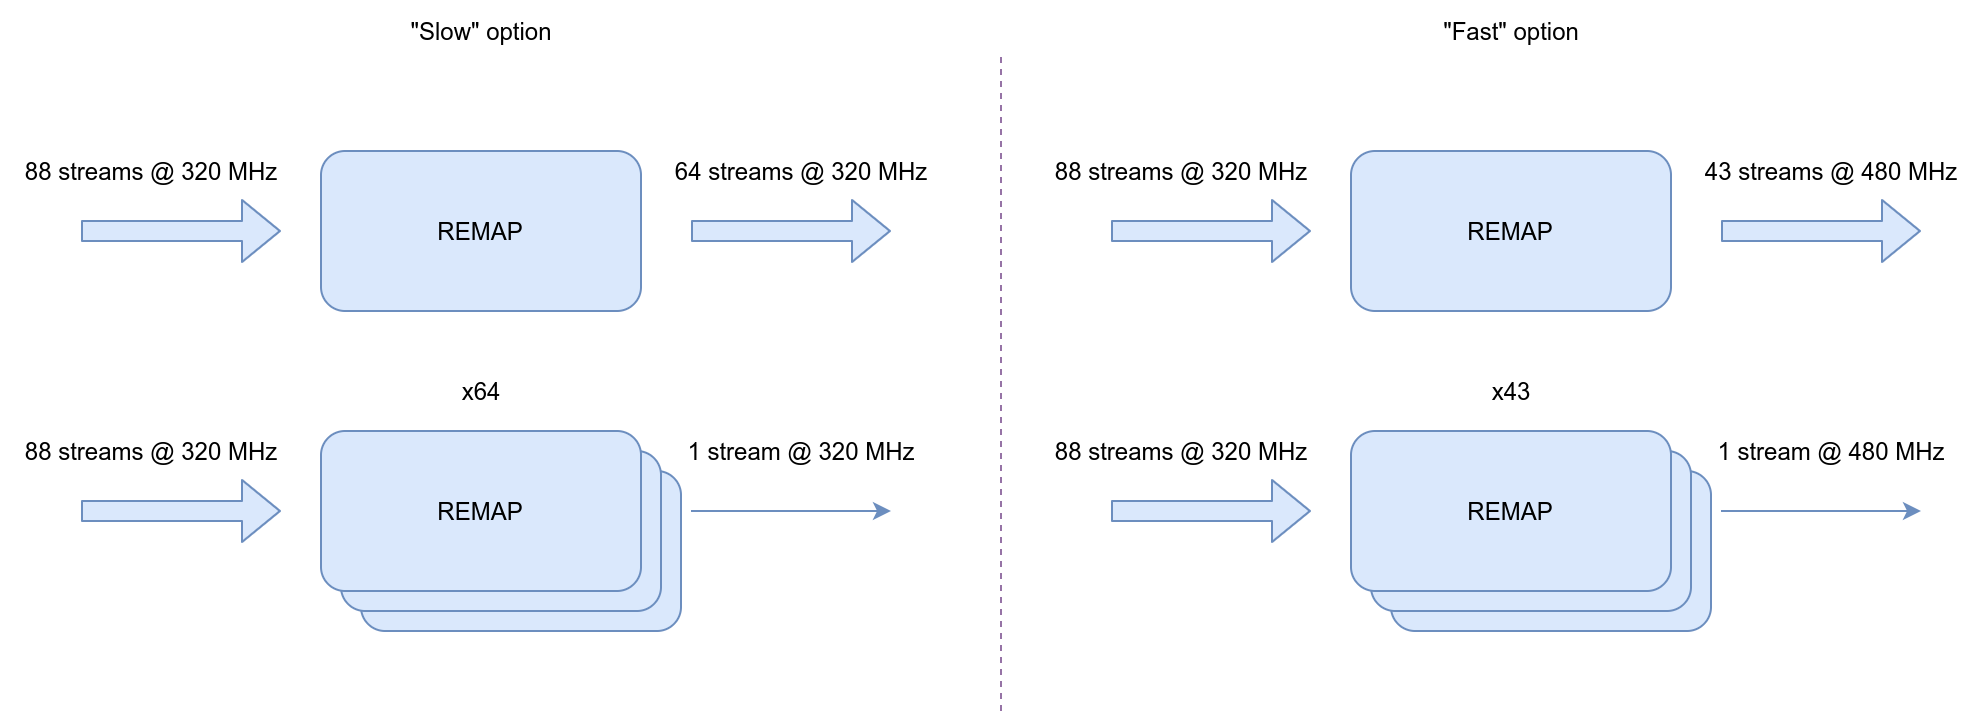
\includegraphics[width=\linewidth]{remap_replication.png}
    \caption{Схема формирования необходимого количества выходных каналов}
    \label{fig:remap_replication}
\end{figure}\par

Стоит отметить, поскольку входной поток данных разбивается на 4 независимые части, обрабатывающиеся отдельно, каждый модуль \texttt{remap} должен принимать лишь 22 канала и формировать 16 или 11 выходов, в зависимости от варианта сигнального процессора LASP.\par
В ходе разработки было спроектировано и реализовано два различных варианта архитектуры базового элемента модуля \texttt{remap}: с модулем синхронизации тактовых доменов, а также архитектура, основанная на FIFO памяти.\par
Во всех вариантах архитектуры можно выделить три основных этапа обработки:\par
\begin{itemize}
    \item предварительная перестановка данных в рамках каждого входного канала;
    \item извлечение из потока интересующих значений и их запись в память;
    \item чтение сохранённых данных из памяти в корректном порядке.
\end{itemize}\par
Первый этап обработки реализуется с помощью внешнего модуля Ialign и заключается в переупорядочивании значений АЦП в пределах каждого отдельного канала данных. Для корректной работы модуля \texttt{remap} требуется подобрать такую конфигурацию этих перестановок по всем каналам, чтобы значения, предназначенные для любого выходного канала не пересекались по временным ячейкам.\par
На втором этапе данные поступают на мультиплексор, который захватывает лишь один канал на каждом из тактов. Именно для этой операции и требуется условие первого этапа -- если одномоментно несколько входных каналов будут содержать значения, предназначенные для одного выходного, то часть данных будет просто пропущена. Это ограничение особенно важно для варианта сигнального процессора LASP с медленной опцией: как на входных интерфейсах, так и на выходных для каждого столкновения пучков передаётся по 8 величин, поэтому крайне необходимо, чтобы на каждом такте было доступно нужное значение. В быстрой опции выходной интерфейс имеет по 12 ячеек с данными, что вынуждает размещать два мультиплексора, ведь одного не будет достаточно в любом случае. В таком раскладе допускается одновременное наличие не более двух активных каналов для каждого базового блока модуля конфигурируемой перестановки. Извлечённые из общего потока значения, предназначенные для определённого выходного канала, временно буферизируются в памяти.\par
После накопления всех необходимых значений АЦП их необходимо переупорядочить, что осуществляется просто путём считывания данных в требуемой последовательности, согласно конфигурации. Стоит отметить, что буферизация данных в памяти позволяет обеспечить их безопасный переход из тактового домена $f_{feb}$ в домен $f_{core}$.\par

\subsubsection{Архитектура с модулем синхронизации тактовых доменов}
Первый вариант архитектуры компонента Remap, содержащий специальный модуль синхронизации тактовых доменов, представлен на рисунке \ref{fig:remap_cds}.\par
\begin{figure}[ht]
    \centering
    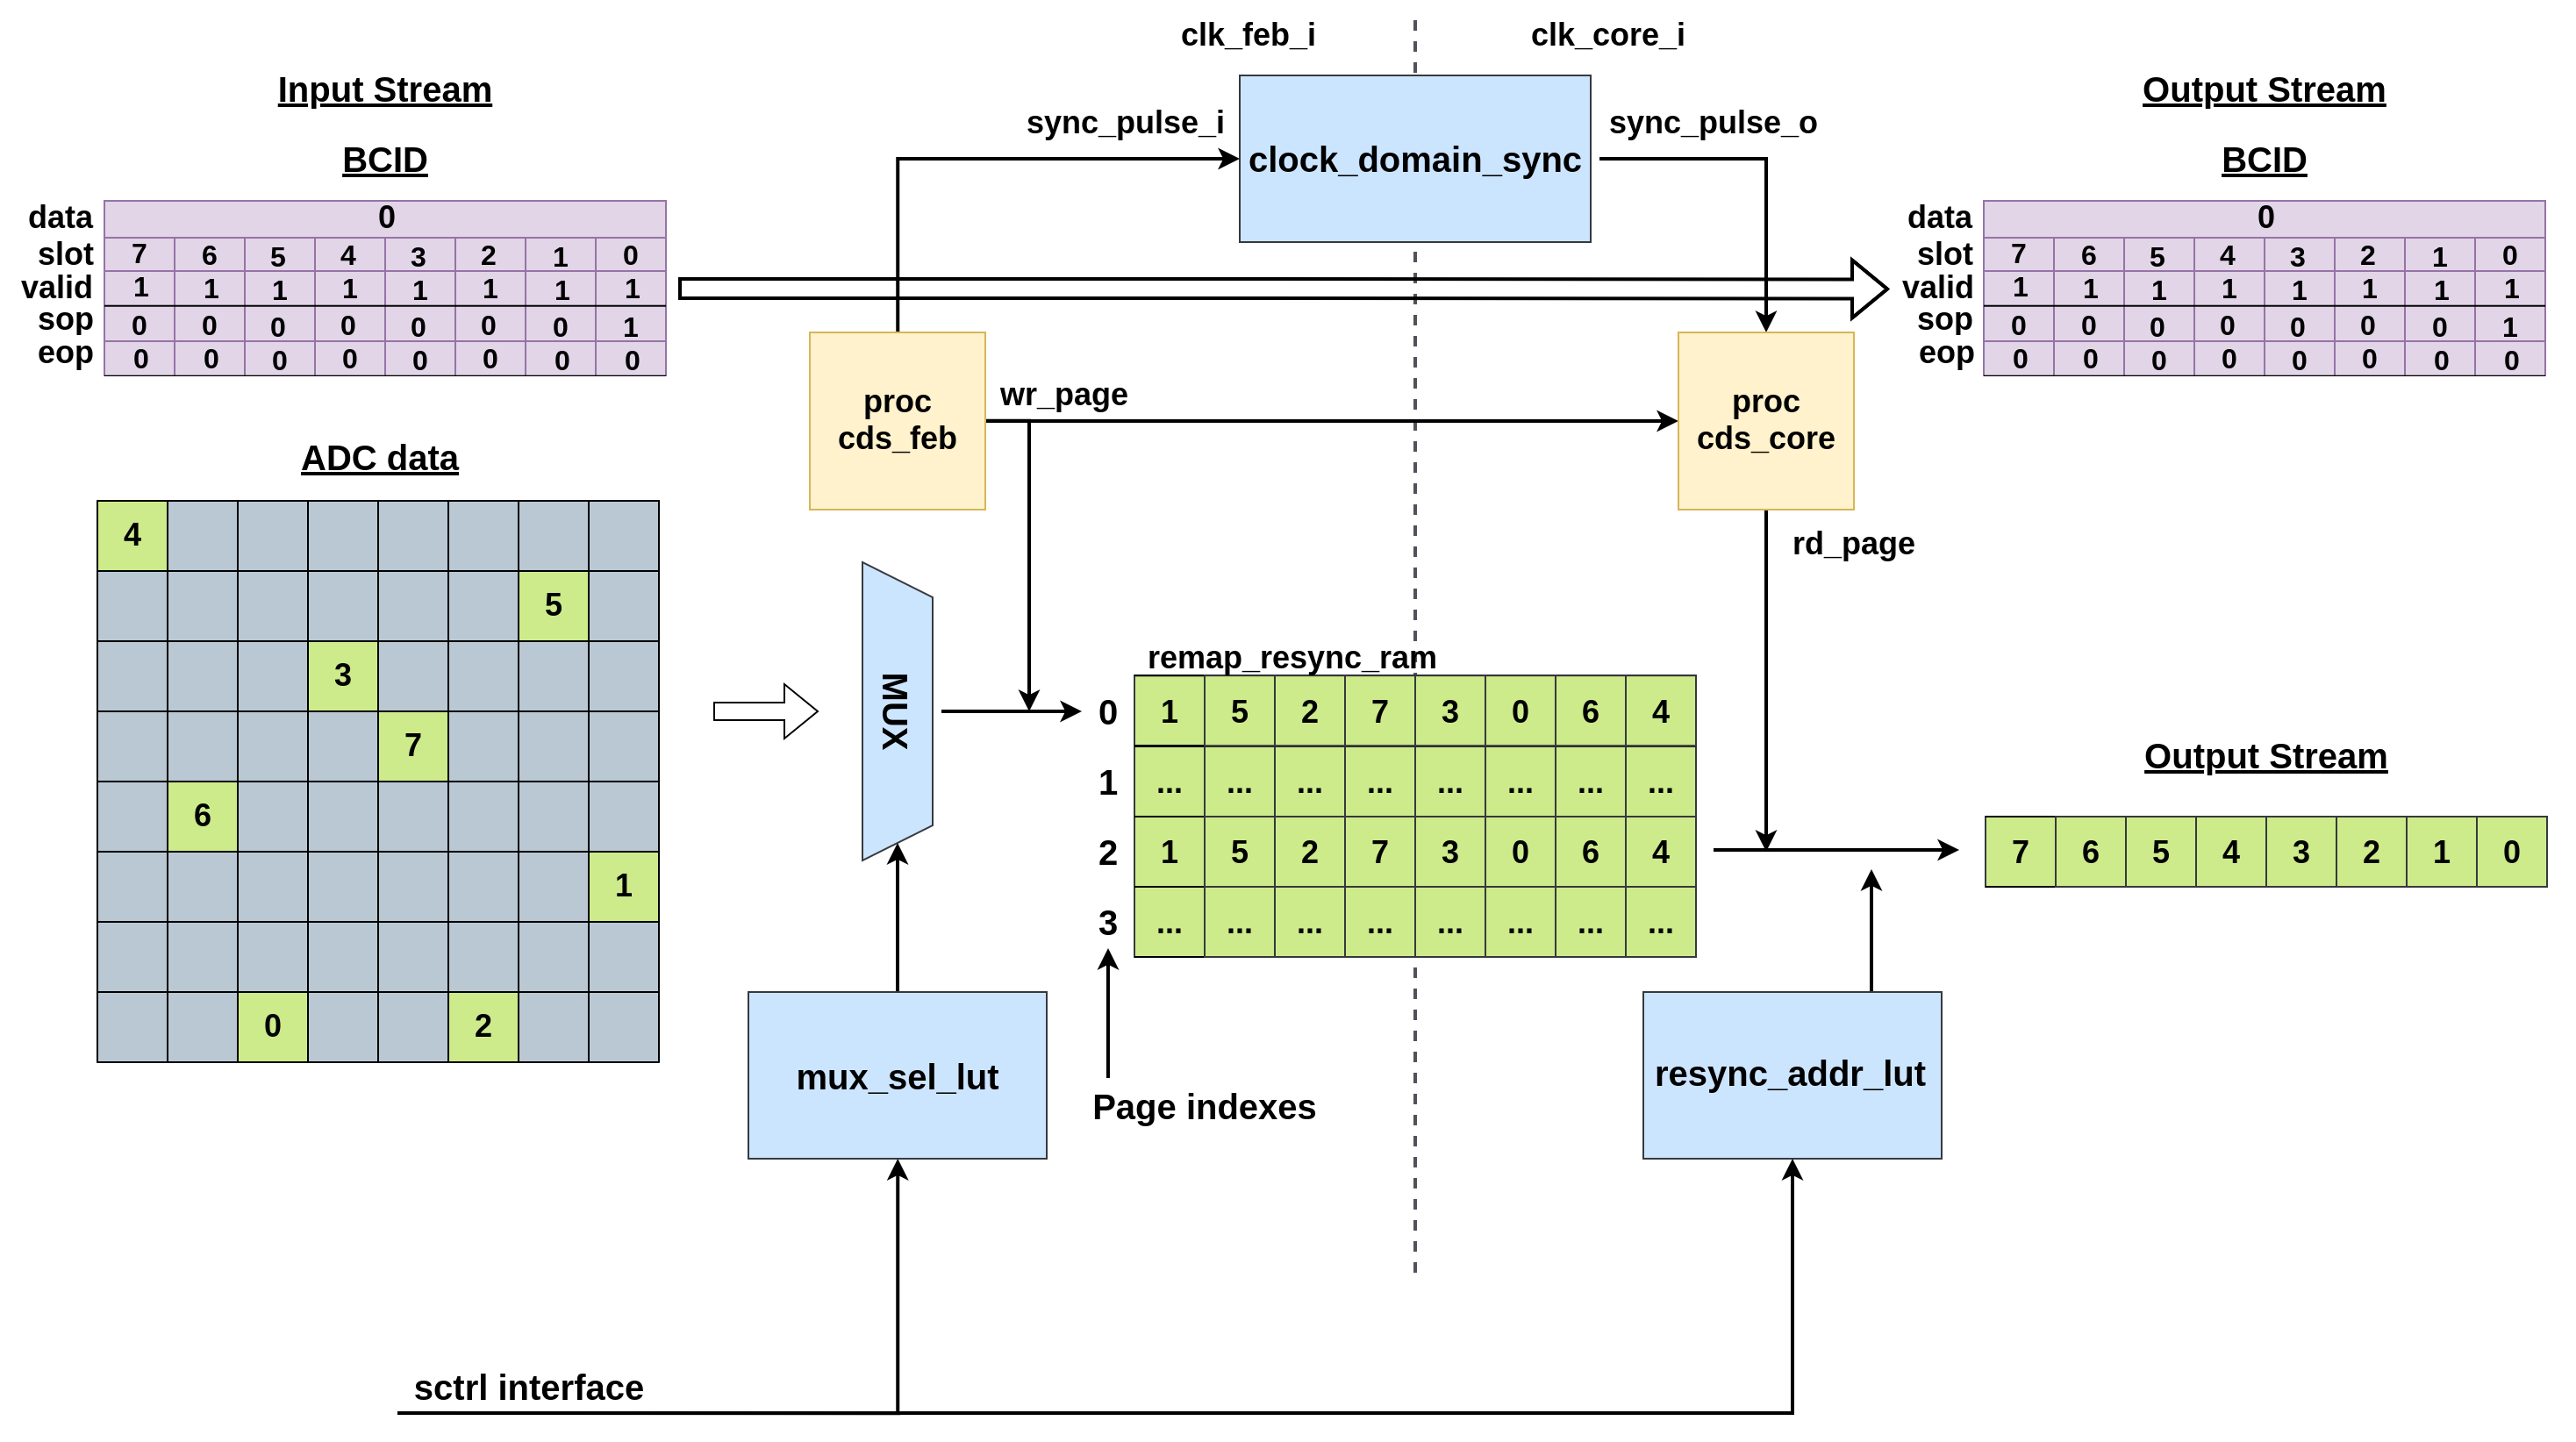
\includegraphics[width=\linewidth]{remap_cds.png}
    \caption{Схема архитектуры модуля Remap с модулем синхронизации тактовых доменов ПЕРЕВЕСТИ}
    \label{fig:remap_cds}
\end{figure}\par
Основной особенностью этой архитектуры является то, что в качестве буфера для мультиплексированных данных используется блок двухпортовой RAM памяти. Эта память разбита на несколько страниц, каждая из которых имеет размер, достаточный для хранения захваченной информации, относящейся к одному столкновению пучков. Чтение данных из страницы начинается лишь только после её полного заполнения записывающей стороной. Для синхронизации процессов считывания и записи предусмотрен следующий механизм: по завершению заполнения страницы памяти записывающая логика генерирует импульс шириной в один такт и отправляет его на вход специального модуля. Внутри этого модуля расположены два счётчика, работающие на тактовых частотах $f_{feb}$ и $f_{core}$, которые ведут счёт в диапазоне количества временных ячеек для каждого BCID. В рабочем режиме первый настроен так, чтобы обнуляться одновременно с поступлением синхросигнала от записывающей логики, а второй с задержкой около такта $f_{feb}$ после первого. При завершении цикла работы второго счётчика формируется выходной сигнал синхронизации, который поступает к считывающей логике и означает, что очередная страница в двухпортовой памяти заполнена полностью и можно безопасно извлекать из неё данные. Если вдруг синхронизация собьётся и синхросигнал от системы записи придёт не вовремя, то модуль это обнаружит и перейдёт в режим восстановления синхронизации. Часть данных после сбоя синхронизации будет утеряно, но через некоторое время система автоматически восстановится и продолжит работать исправно.\par
Описанная архитектура была реализована на языке описания цифровой логики VHDL и отлажена. По результатам тестирования в симуляторе она подтвердила свою работоспособность. Однако такой подход имеет ряд недостатков, главным из которых является необходимость передавать целый набор сигналов(такие как номер текущей страницы, индекс столкновения пучка, а также ряд вспомогательных сигналов внутри модуля синхронизации тактовых доменов) между тактовыми доменами $f_{feb}$ и $f_{core}$ вручную, используя схемы на двух регистрах. Для корректной организации таких переходов требуется тонкая ручная настройка временных ограничений, реализуемая путём составления специальных указаний синтезатору физической схемы, входящему в состав программного комплекса Intel Quartus Prime. Это значительно усложняет весь проект и делает его гораздо менее гибким. После возникновения проблем с разводимостью логики проекта LATOME, который является основой задетекторной электроники эксперимента ATLAS, разработанной в рамках предшествующей фазы обновления детектора, командой разработчиков сигнального процессора LASP было принято решение максимально избегать подобные способы перехода между тактовыми доменами. Кроме того, данный вариант является довольно путанным и сложным для понимания в деталях. Учитывая все эти недостатки, было решено разработать альтернативную архитектуру модуля Remap.\par


\subsubsection{Архитектура, основанная на FIFO}
Второй вариант архитектуры компонента Remap, содержащий память FIFO, представлен на рисунке \ref{fig:remap_fifo}.\par
\begin{figure}[ht]
    \centering
    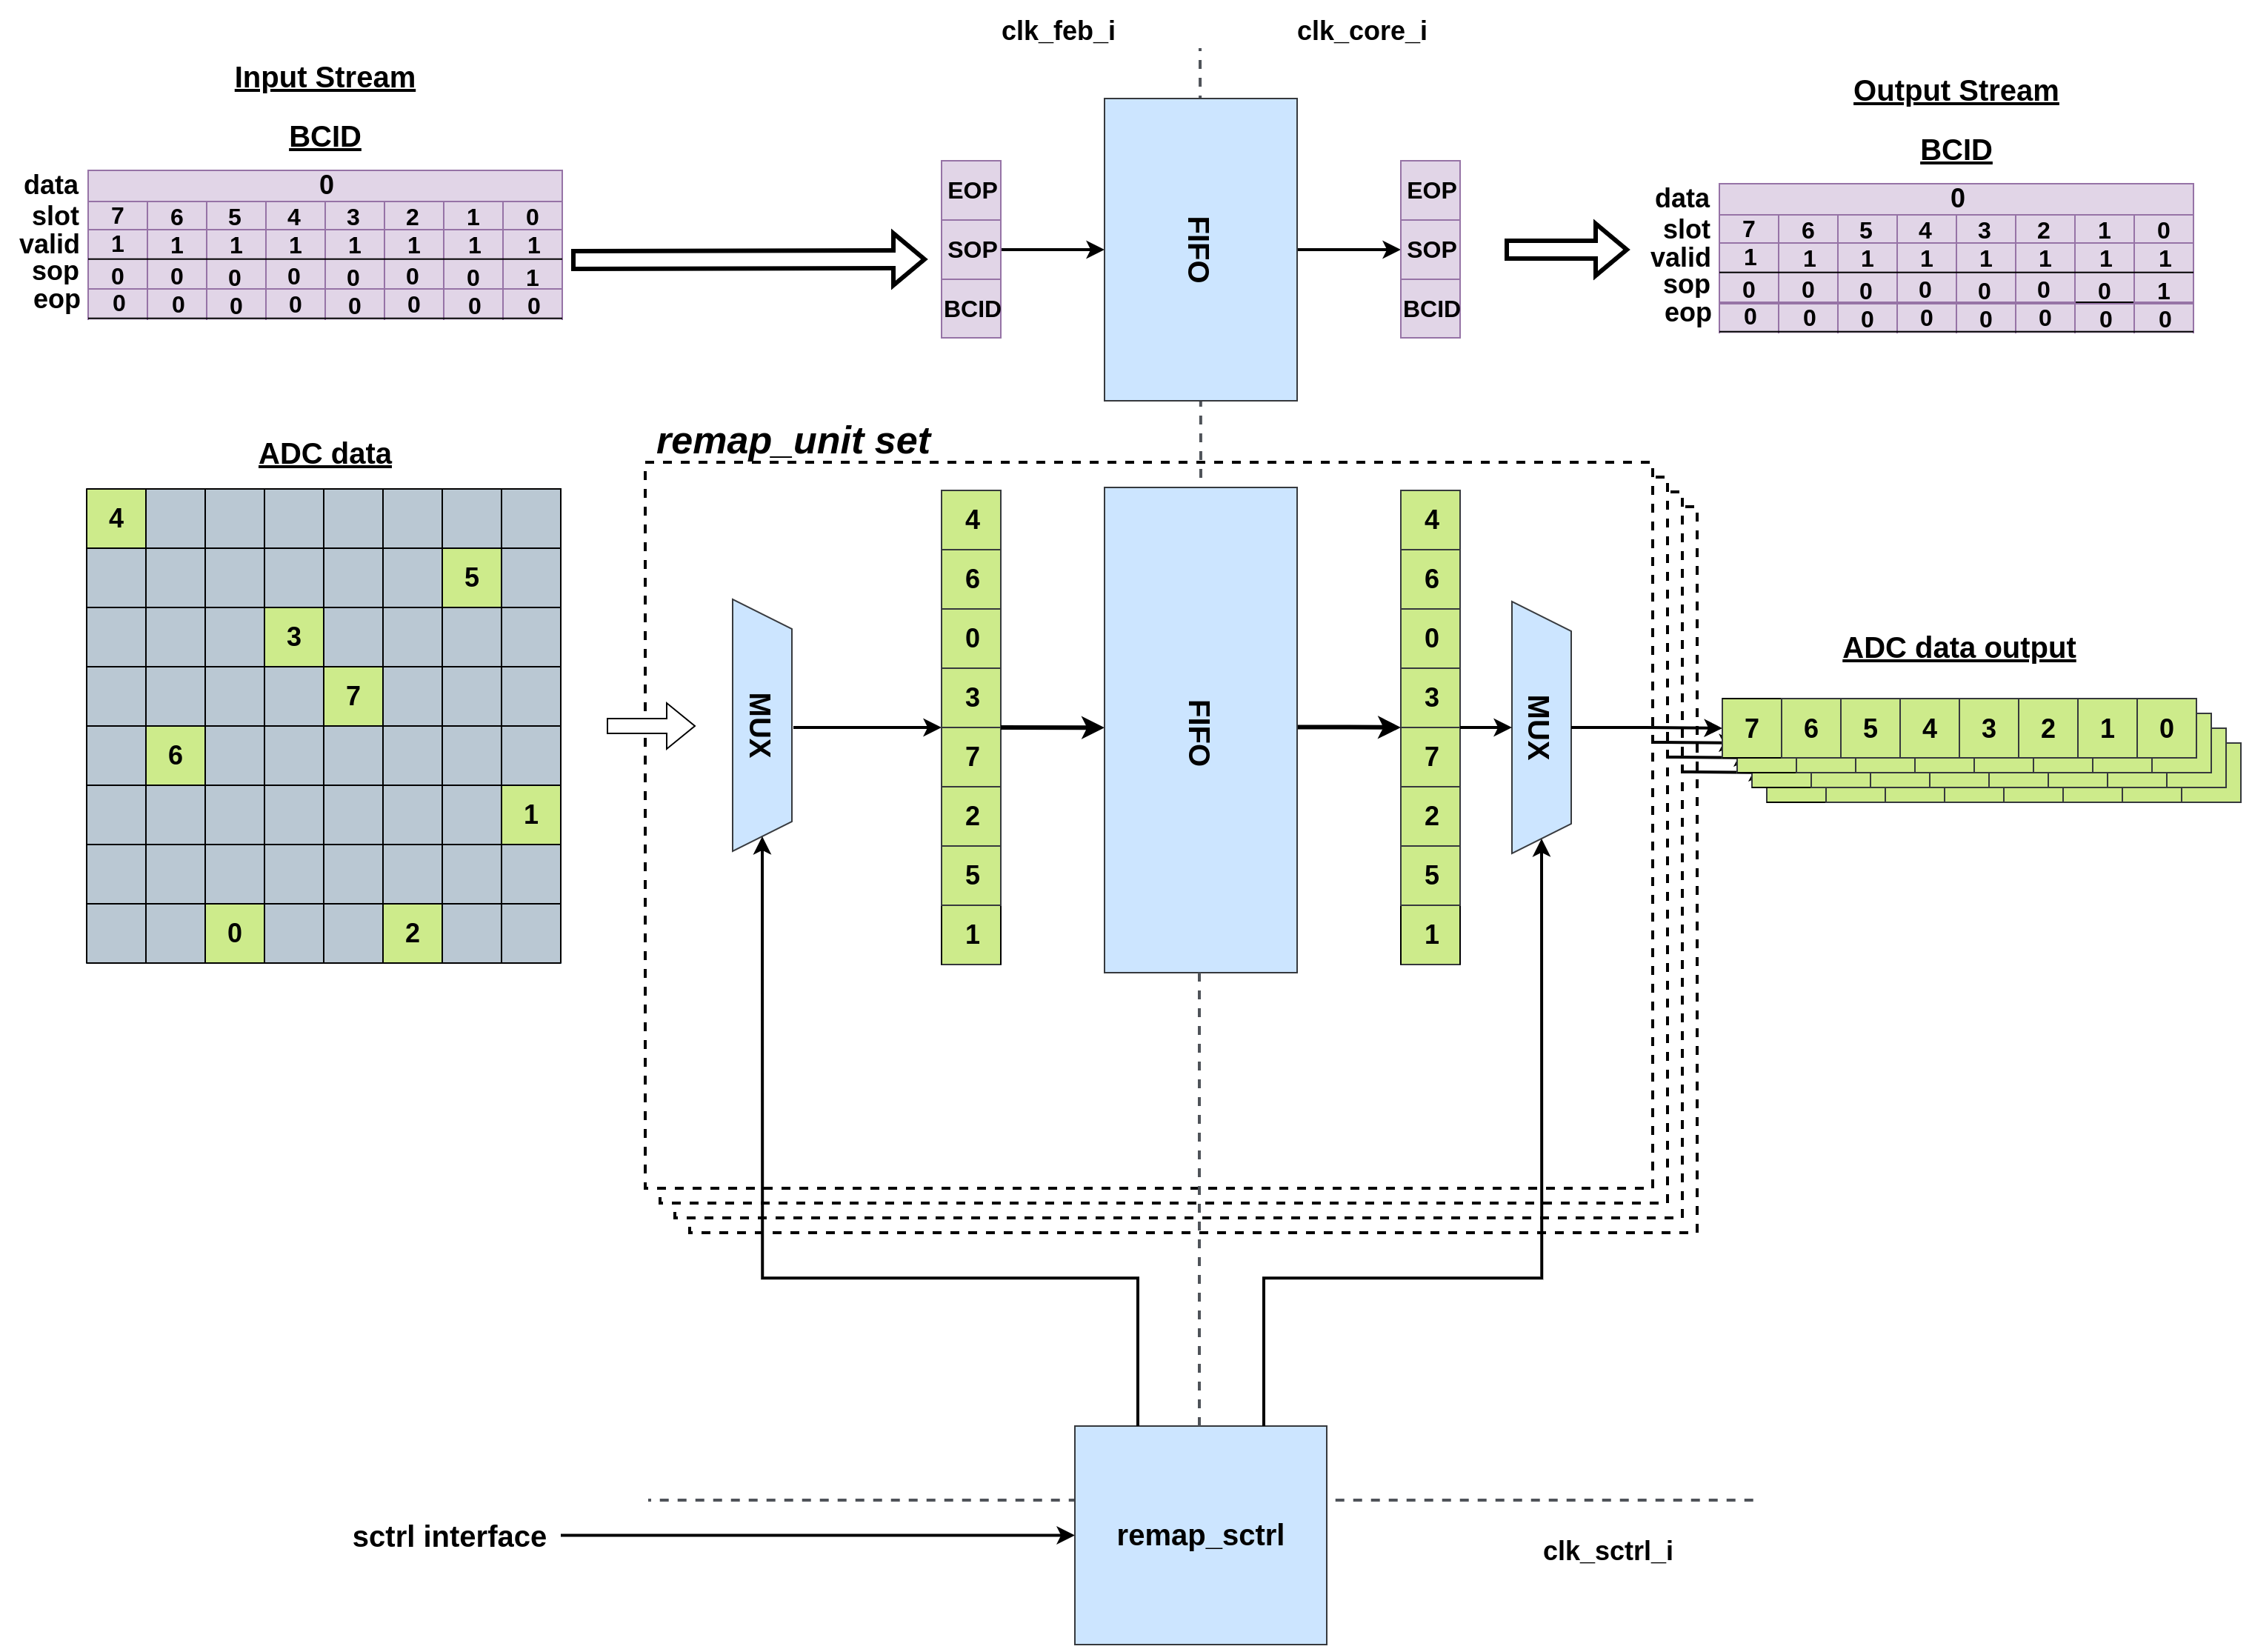
\includegraphics[width=\linewidth]{remap_fifo.png}
    \caption{Схема архитектуры модуля Remap, основанной на FIFO ПЕРЕВЕСТИ}
    \label{fig:remap_fifo}
\end{figure}\par
В рамках данного подхода в качестве буфера для мультиплексированных данных является память FIFO (First In First Out). Такая структура состоит из двухпортовой памяти, двух счётчиков адреса и двух автоматов для чтения и записи данных и является одним из ключевых элементов цифровой схемотехники. Одно из самых распространённых применений такой памяти, помимо буферизации информации -- это реализация перехода данных между тактовыми доменами. Поскольку такая память используется невероятно часто в проектировании логических схем, то существует множество готовых вариантов их реализации, в том числе и от разработчиков самих микросхем ПЛИС и соответствующего программного обеспечения для автоматического проектирования, в том числе и от Intel. В случае использования такого готового блока FIFO не требуется ручное написание временных ограничений, что избавляет от потенциальных проблем на этапе синтеза цифровой схемы всего проекта.\par
Однако, одна из основных особенностей FIFO -- это сохранение порядка записываемых данных, что не позволяет реализовать последний этап работы модуля Remap. Для решения данной задачи используется подход, при котором данные с мультиплексора поступают не напрямую на вход FIFO, а записываются в один большой регистр, достаточного размера для одновременного хранения всех мультиплексированных данных в рамках текущего столкновения пучков. Для наиболее оптимального использования логических ресурсов этот регистр является сдвиговым, то есть каждый такт новое значение поступает в начало, после чего оно смещается дальше. Только после полного заполнения этого регистра актуальными величинами, данные одним большим словом записывается в FIFO. Считывающая логика, после обнаружения данных на выходе FIFO, имеет доступ сразу ко всем значениям и может извлекать их последовательно в необходимом порядке.\par
В целях минимизации латентности необходимо, чтобы поступающие в FIFO данные сразу же были доступны для чтения, то есть требуется не допускать его заполнения. Поскольку запись и извлечение идёт с одной и той же скоростью, важно важно сделать так, чтобы считывающая система начала работу как минимум не позднее записывающей. Это достигается правильным управлением сигналами сброса: после старта сигнального процессора LASP сначала должен сняться сброс, синхронный с тактовым доменом $f_{core}$, а уже затем $f_{feb}$.\par



\subsection{Конфигурирование через интерфейс медленного контроля}
Конфигурирование модуля \texttt{remap} осуществляется через интерфейс медленного контроля. Как упоминалось ранее, он функционирует поверх протокола Avalon Memory Mapped, который предназначен для работы с адресуемой памятью. Такой подход очень удобен, поскольку в этом случае можно выделить каждому модулю свой участок адресов, по которым можно будет располагать необходимые значения. Разные адреса можно настроить по способу доступа к ним, таким образом можно завести некоторые показатели системы, которые можно будет только считывать, или же добавить параметры с опцией модификации. Отдельная важная особенность работы через память -- возможность функционирования в разных тактовых доменах, для этого достаточно использовать модули двухпортовой памяти. Это позволяет использовать достаточно низкую тактовую частоту для интерфейса конфигурации, чтобы он не оказывал существенного влияния на разводимость остальной логики. Причём эта частота может быть единой для конфигурирования всех компонентов, вне зависимости от их внутренних тактовых сигналов, что значительно упрощает работу медленного контроля.\par
Модуль перестановки \texttt{remap} имеет две конфигурируемые стадии: какие значения извлекать из общего потока данных с помощью мультиплексора и в каком порядке их выдавать в выходной канал. Поскольку эти стадии работают в разных тактовых доменах, то необходимо размещать параметры для них в разных блоках памяти, чтобы можно было корректно переводить значения в целевые тактовые частоты. Начальный адрес конфигурации мультиплексора устанавливается глобальной константой REMAP\_BADDR (Remap Base Address) с уровня всего проекта сигнального процессора LASP, а конфигурация порядка выходных данных имеет некоторое смещение относительно него. На рисунке \ref{fig:remap_sctrl_mapping} изображена схема отображения конфигураций на адресное пространство.\par
\begin{figure}[ht]
    \centering
    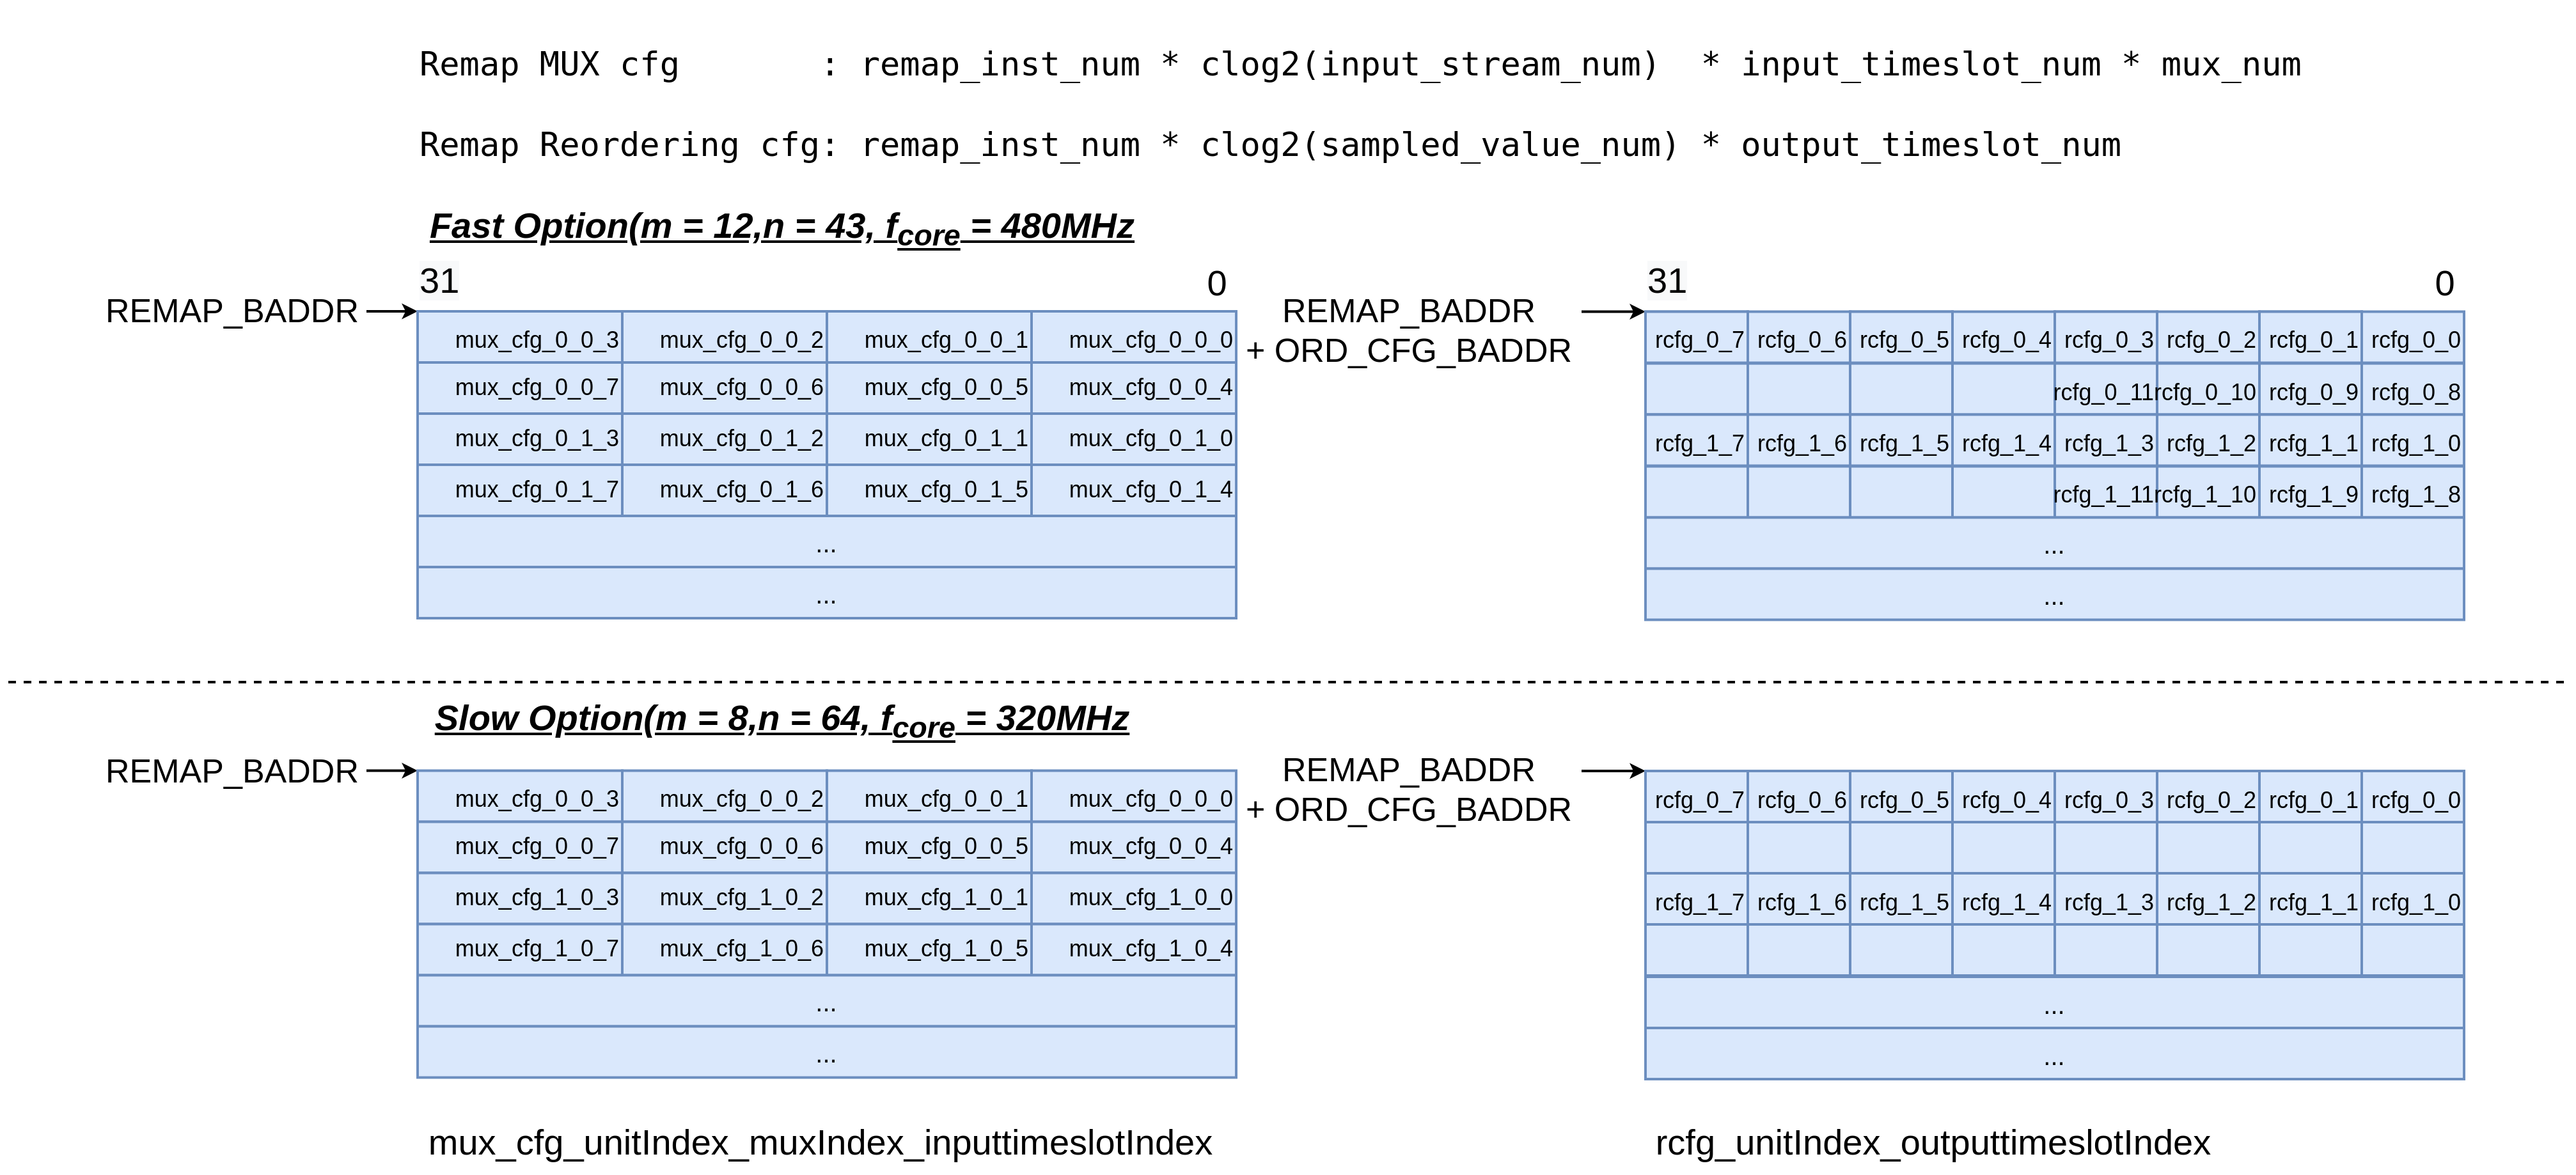
\includegraphics[width=\linewidth]{remap_sctrl_mapping.png}
    \caption{Схема маппинга памяти модуля перестановки \texttt{remap} для записи конфигурации}
    \label{fig:remap_sctrl_mapping}
\end{figure}\par
Для конфирурирования входного мультиплексора необходимо для каждой временной ячейки установить номер канала, с которого необходимо захватить данные. На каждый \texttt{remap} поступает по 22 канала, то есть требуется 5 бит на значение. Для любого столкновения пучков выделяется по 8 временных интервалов, следовательно суммарно должно быть не менее 40 бит данных для конфигурирования одного выходного канала \texttt{remap}. Шина данных интерфейса Avalon Memory Mapped имеет ширину 32 бита, поэтому для удобства формирования и чтения конфигурационных данных используется 2 слова AVMM, что составляет 64 бита. В случае варианта быстрой опции сигнального процессора LASP требуется два входных мультиплексора, соответственно размер конфигурации удваивается и равняется 128 бит.\par
Конфигурирование финальной перестановки осуществляется путём последовательного указания индекса необходимого значения. В зависимости от медленной или быстрой опции отобранных величин может быть 8 или 16 соответственно. Для более удобной работы под каждое такое значение выделяется по 4 бита. Далее, в зависимости от варианта сигнального процессора LASP требуется от 8 до 12 временных ячеек для каждого BCID, следовательно суммарно необходимо иметь от 32 до 48 бит. Аналогично конфигурации мультиплексора, в целях повышения удобства размер конфигурации округляется по ширине шины интерфейса AVMM и составляет 64 бита независимо от опции сигнального процессора LASP.\par


\subsection{Реализация}

\subsubsection{Симуляция}
В ходе реализации синтезируемых компонентов модуля Remap активно использовалось тестирование с помощью симуляции. Оно осуществлялось с помощью специализированного программного обеспечения Mentor QuestaSim, предназначенное для моделирования и отладки микросхем ПЛИС. Симуляционное окружение разработано, как и синтезируемые модули, на языке VHDL и обеспечивает поступление данных на входной интерфейс тестируемого модуля. Так, на рисунке \ref{fig:sim_input} приведён фрагмент симуляции, на котором показан пример данных внутри внутри  входного интерфейса. Можно увидеть, что как и в реальной системе, в каждый модуль Remap поступает 22 канала со значениями АЦП, причем для каждого BCID передаётся по 8 величин в канале. Все сигналы входного сигнала синхронны с тактовой частотой $f_{feb}$.\par
\begin{figure}[ht]
    \centering
    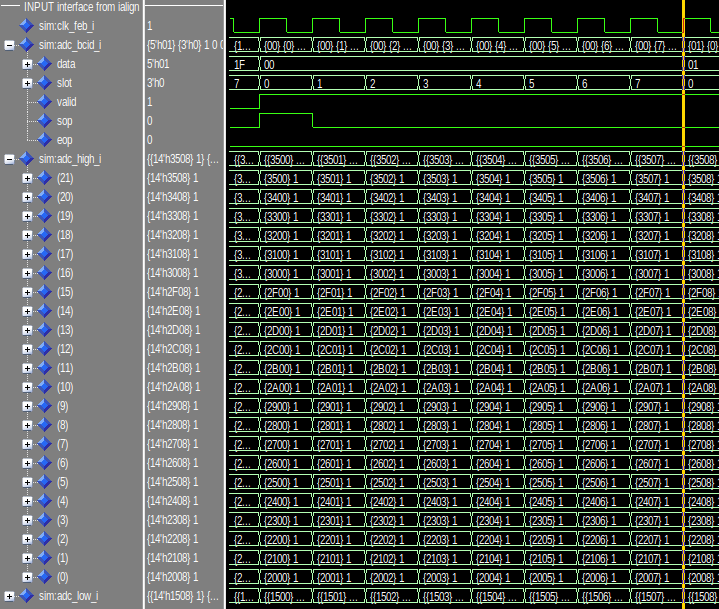
\includegraphics[width=\linewidth]{sim_input.png}
    \caption{Фрагмент поступающих в модуль Remap входных данных в симуляции}
    \label{fig:sim_input}
\end{figure}\par
В рассматриваемом примере модуль предназначен для работы в варианте сигнального процессора LASP с установленной медленной опцией. В качестве конфигурации производится установка параметров для первых двух выходных каналов Remap компонента. На рисунке \ref{fig:sim_sctrl} отображено, как это осуществляется через интерфейс медленного контроля. На волновой диаграмме отчетливо видно, как значения поступают в установленном формате по протоколу AVMM, после чего лишние биты отсекаются, а сами конфигурационные данных переходят в соответствующие им тактовые домены. В соответствии с настройкой, первый выходной канал должен выдавать данные из первых восьми входных каналов в обратной последовательности, а второй по четыре значения из каналов с номерами 20 и 21 в чередующейся последовательности.\par
\begin{figure}[ht]
    \centering
    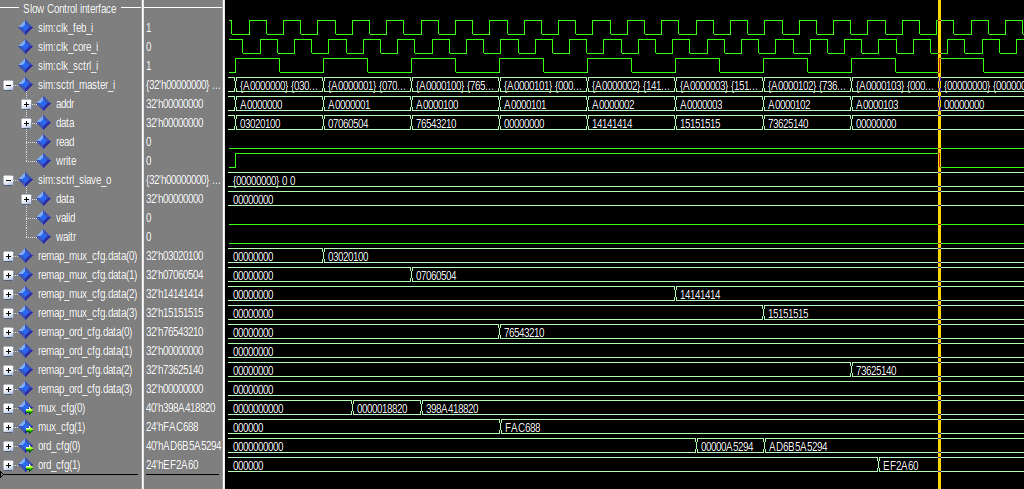
\includegraphics[width=\linewidth]{sim_sctrl.png}
    \caption{Пример записи конфигурации модуля Remap в симуляции}
    \label{fig:sim_sctrl}
\end{figure}\par
На рисунке \ref{fig:sim_output} изображен выходной интерфейс модуля конфигурируемой перестановки. Поскольку система предназначена для работы в медленной опции сигнального процессора LASP, выходной интерфейс состоит из 16 каналов, в котором данные передаются синхронно частоте $f_{core}$, равной 320 МГц. На нём можно отследить корректность работы компонента, работающего в соответствии с вышеописанными настройками. \par
\begin{figure}[ht]
    \centering
    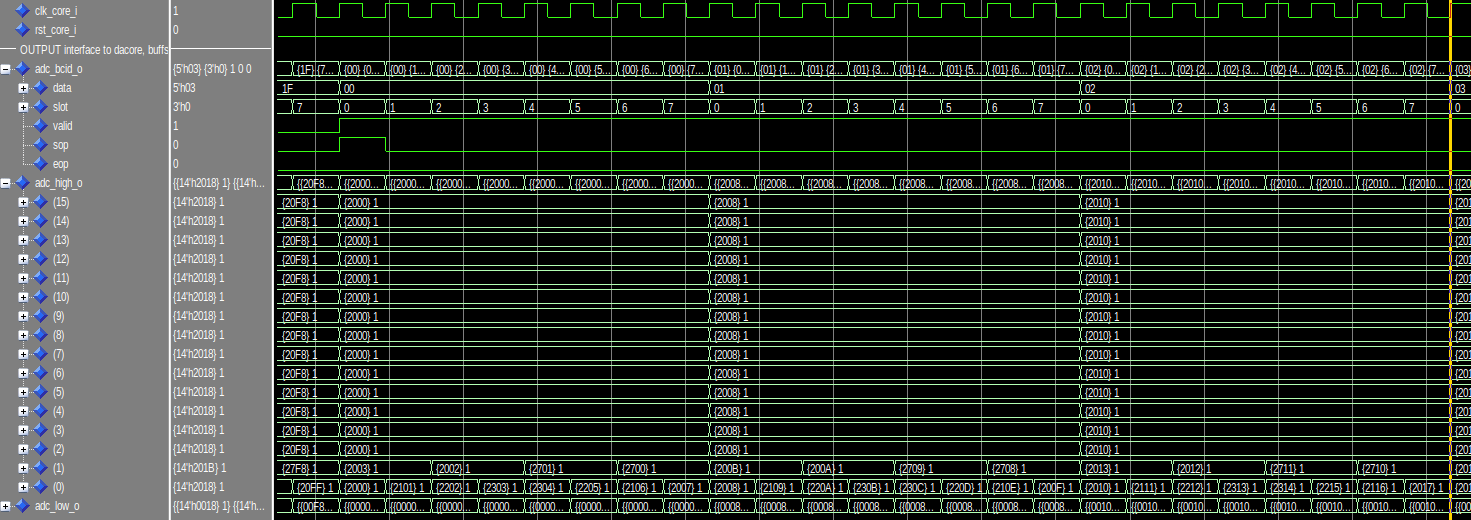
\includegraphics[width=\linewidth]{sim_output.png}
    \caption{Фрагмент выходящих из модуля Remap данных в симуляции}
    \label{fig:sim_output}
\end{figure}\par


\subsubsection{Синтез}
После отладки функциональности в симуляторе был произведён синтез модуля \texttt{remap} под платформу КАКАЯ в обоих вариантах конфигурации сигнального процессора LASP. В таблице \ref{tab:remap_util} представлены значения используемых логических ресурсов для синтеза модуля, рассчитанного под обработку 22 входных каналов данных. Количество выходных каналов, в свою очередь, зависит от опции LASP.\par
\begin{table}[ht]
    \caption{Используемые модулем remap логические ресурсы}
    \begin{tabular}{|p{0.3\textwidth}|p{0.3\textwidth}|p{0.3\textwidth}|}
        \hline
        Тип & Медленная опция & Быстрая опция \\
        \hline
        ALM & 3077 & 2249 \\
        \hline
        ALUT & 1728 & 1686 \\
        \hline
        Регистры & 7075 & 4530 \\
        \hline
        block mem bits & 7168 & 2600 \\
        \hline
        Блоки памяти M20K & 76 & 37 \\
        \hline
    \end{tabular}
    \label{tab:remap_util}
\end{table}
По таблице отчетливо видно, что модуль использует меньше логических ресурсов ПЛИС при работе в быстрой опции, поскольку в таком варианте необходимо генерировать меньшее количество выходных каналов, но на более высокой частоте. С точки зрения временных ограничений, обе версии модуля \texttt{remap} синтезируются без проблем и имеют запас по установке сигнала в 350 и 260 пикосекунд соответственно. Задержка при передаче данных составляет порядка 30 наносекунд, что удовлетворяет требованиям, предъявляемых модулю.\par




\subsection{Программное обеспечение}
В целях автоматизации процесса формирования конфигураций для модулей \texttt{remap} велась разработка соответствующего программного обеспечения. Первым делом в ручном режиме была изучена структура входных данных и сформирован профиль переупорядоченных данных выходного интерфейса. Для каждого участка жидкоаргонового калориметра существует карта, согласно которой оцифрованные значения АЦП поступают в сигнальный процессор LASP. Они представлена в виде таблиц, каждая из которых состоит из 88 строк и 6 колонок, в соответствии с количеством подключаемых входных каналов и временных ячеек для передачи данных в рамках каждого канала. Каждая ячейка содержит аббревиатуру, несущую в себе полную информацию об источнике сигнала. Поскольку калориметры имеют некоторую регулярность в своей структуре, то из всех четырёхсот карт можно выделить всего двадцать уникальных, в которых структура входных данных является действительно уникальной. То есть достаточно составить двадцать схем перестановок, и применить одну из них для каждой из существующих. Пример карты упорядочивания входных значений для участка цилиндрической части жидкоаргонового калориметра изображен на рисунке \ref{fig:remap_remapping}. При составлении выходной карты данных в первую очередь преследовалось удобное расположение данных для последующего вычисления сумм по участкам калориметра.\par
\begin{figure}[ht]
    \centering
    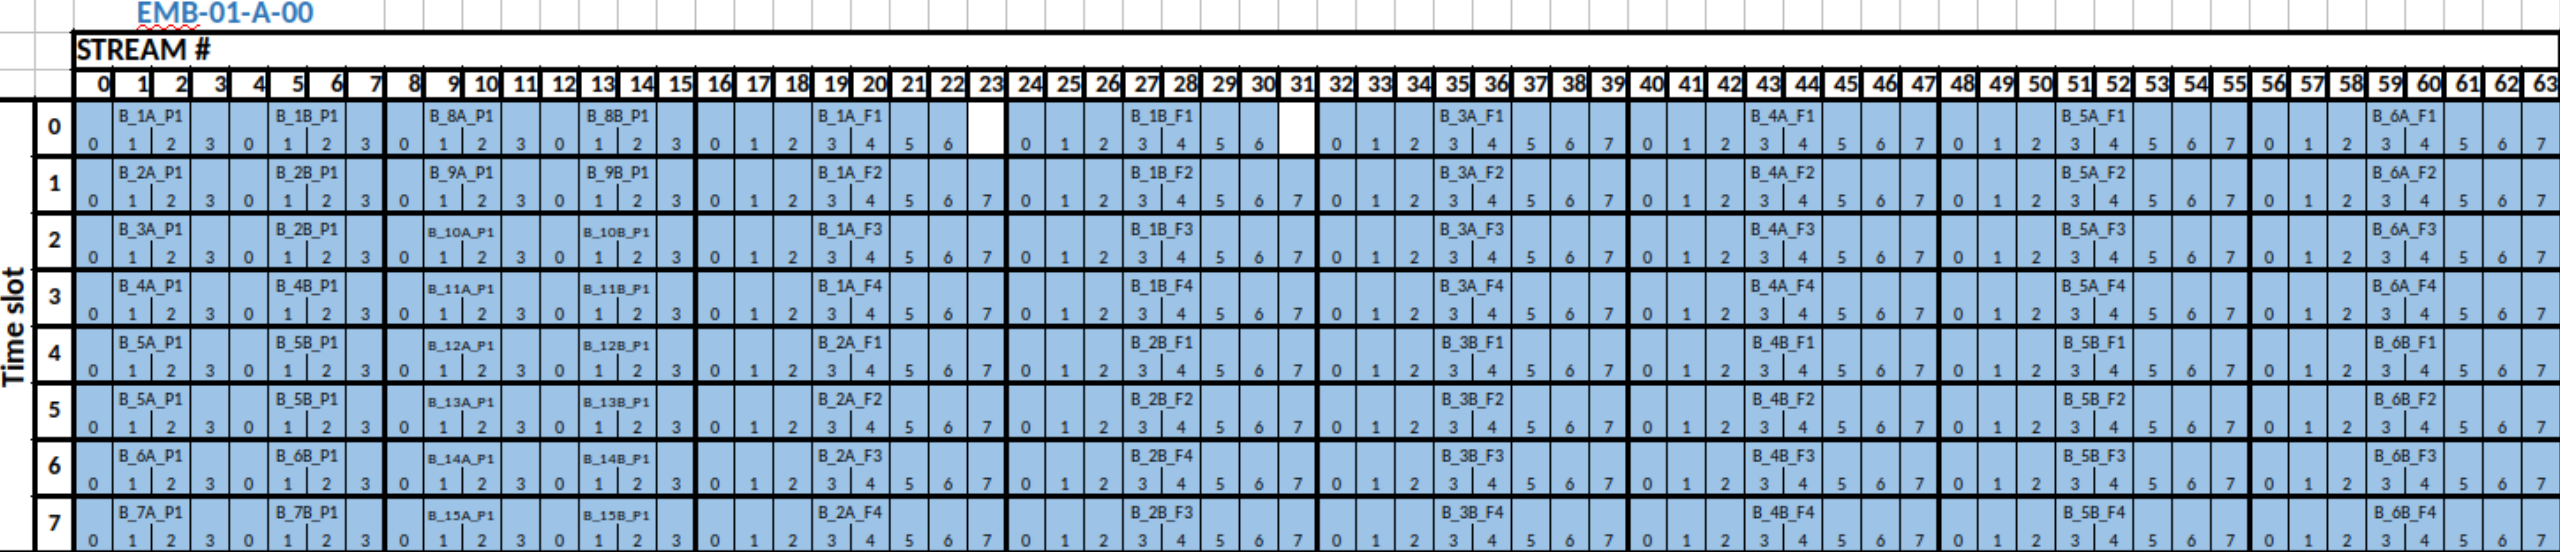
\includegraphics[width=\linewidth]{remap_remapping.png}
    \caption{Пример схема упорядочивания выходных данных модуля remap}
    \label{fig:remap_remapping}
\end{figure}\par
С помощью скрипта написанного на языке Python выполняется автоматическая генерация конфигурационных значений для модуля \texttt{remap}. Первый этап его работы заключается в подборе такого порядка значений внутри каждого отдельного входного канала, который обеспечивал бы отсутствие пересечений данных, предназначенных для каждого выходного канала, по временным ячейкам. Эти перестановки предназначаются для реализации модулем \texttt{ialign}. Следующим этапом является поиск последовательности номеров входных каналов, необходимых мультиплексирования каждой секцией модуля \texttt{remap}. Заключительным этапом является формирование набора чисел, согласно которым отобранные мультиплексором данные будут упорядочены. Значительным упрощением является тот факт, что входные каналы данных разбиваются на четыре независимых набора, следовательно и конфигурации составляются не по всем 88 каналам, а только по 22.\par
В настоящий момент разработка данного ПО не завершена, поскольку реализован лишь прототип, который работает с одним минимальным набором из 22 входных каналов. После отладки предстоит его масштабирование для работы со всеми участками жидкоаргоновых калориметров.\par

